% 2009 年福建卷文科第 8 题：偶函数 f(x) 在 [0,2] 上的部分图象。
% 来源 PDF：普通高考/2009/2009福建文.pdf，SHA-256 f0a5111a6f86f4d4e8618c5c2cd0ecfd678a590b36ecbd033bb63b189700a0bc。
% 原页：第 1 页（A3 三栏）第 2 栏中部，书页码 517。
% 重绘依据：按原页示意曲线重绘，只画 [0,2] 一段，x=2 处虚线，标出 (0,1) 与 2。
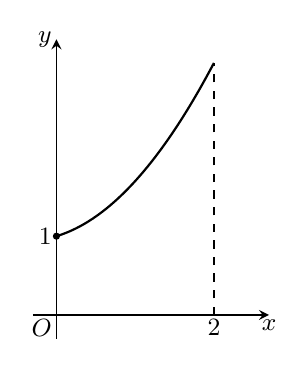
\begin{tikzpicture}[semithick, every node/.style={inner sep=1.4pt, font=\small}]
  \draw[-stealth] (-0.3,0) -- (2.7,0) node[below] {$x$};
  \draw[-stealth] (0,-0.3) -- (0,3.5) node[left] {$y$};
  \node[below left] at (0,0) {$O$};
  \fill (0,1) circle (1.3pt);
  \node[left] at (0,1) {$1$};
  \draw[thick,domain=0:2,samples=80] plot (\x,{1+0.30*\x+0.40*\x*\x});
  \draw[dashed] (2,0) -- (2,{1+0.30*2+0.40*4});
  \node[below] at (2,0) {$2$};
\end{tikzpicture}
